\documentclass[12pt]{article}
\usepackage{geometry}
\usepackage{gensymb} %grādu simbols
\usepackage[utf8]{inputenc}
\usepackage{tcolorbox}
\usepackage{multicol}
\usepackage{enumitem}
\usepackage{fancyhdr}
\usepackage{indentfirst}
\usepackage[bf,center]{titlesec}
\usepackage{tocloft}
\usepackage{hyperref}
\usepackage{tabularx}
\usepackage{ragged2e}
\usepackage{tocloft}
\usepackage{secdot}

\hypersetup{
	colorlinks=true,
	linkcolor=black,  
	urlcolor=blue
}

\urlstyle{rm}

\titlespacing*{\section}{0pt}{0pt}{1.5pt}
\titlespacing*{\subsection}{0pt}{0.5\baselineskip}{1.5pt}
\titlespacing*{\subsubsection}{0pt}{0.5\baselineskip}{1.5pt}
\titleformat{\section}{\large \bfseries \centering}{\thesection.}{1em}{}%section formatting
\titleformat{\subsection}{\normalsize \bfseries
	\centering}{\thesubsection.}{1em}{}%subsection formatting
\titleformat{\subsubsection}{\normalsize \bfseries
	\centering}{\thesubsubsection.}{1em}{}%subsubsection formatting
\geometry{a4paper, left=3cm, right=2cm, top=2cm, bottom=2cm}
\pagestyle{fancy}
\fancyhead{}
\fancyfoot{}
\fancyfoot[R]{\thepage}
\renewcommand{\headrulewidth}{0pt}
\linespread{1.3}
\setlength{\parindent}{1cm}
\setlength{\parskip}{0pt}
\renewcommand{\contentsname}{\hspace*{\fill}\bfseries\large Satura rādītājs\hspace*{\fill}} 
\renewcommand{\cfttoctitlefont}{\centering\bfseries\large}% Remove \bfseries from ToC title
\renewcommand{\cftsecfont}{}% Remove \bfseries from section titles in ToC
\renewcommand{\cftsecpagefont}{}% Remove \bfseries from section titles' page in ToC
\renewcommand{\cftsecleader}{\cftdotfill{\cftsecdotsep}}
\renewcommand\cftsecdotsep{\cftdot}
\renewcommand\cftsubsecdotsep{\cftdot}
\renewcommand{\cftsecaftersnum}{.}%dot after section number
\renewcommand{\cftsubsecaftersnum}{.}




\title{Prakses Atskaite}
\author{Māris Muižnieks}





\begin{document}
	\begin{titlepage}
		\thispagestyle{empty}
		\begin{center}
			\vspace*{2cm}
			\begin{large}\textbf{Mācību Centrs MP}
				
				\textbf{Programēšanas Tehniķis 2. Kurss}
				
				\vfill
				\textbf{Prakses Atskaite}
				\textbf{Gameboy Emulātors}
			\end{large}
			
			\vfill
			
		\end{center}
		\vspace{4cm}
		\begin{flushright}
			Autors: \textbf{Māris Muižnieks}
			
			%Darba vadītāja:
		\end{flushright}
		\vspace{1cm}
		\begin{center}
			RĪGA 2022
		\end{center}
	\end{titlepage}
	\tableofcontents
	\pagebreak
	
	\section{Ievads}
	Praksēs mērķis veikt patstāvīgu darbu un pierādīt savas spējas strādāt patstāvīgi, pildīt uzdevumus, izmantot teorētiskās zināšanas praktiskā darbā un pilnveidot tās.
	
	Prakses laikā strādāju SIA "Magnetic Professional" mācību centrs MP, reģ. Nr. 42103086895. 
	
	Prakses uzdevums bija izveidot GameBoy Emulātoru. Prakses laiks no 2022. gada 16. marta līdz 2022. gada 9. maijam. Prakses apjoms 240 Akadēmiskās stundas. 

	Programmēšanai tika izmantota C11 valoda, kā arī SDL2 bibliotēka. Emulātors tika veidots uz Mac OS Monterey 12.2 versīja. Kā arī clang 13.0.0. 
	
	Šajā dokumentā aprakstīšu progamas izveidi, izmantotos informācījas resursus. Problēmas ar kurām sastapos, dažus no risinājumiem. Rīkus un sistēmas kuras izmantoju, kā arī secinājumus, piebildes un ietekumus.

	\pagebreak
	
	\section{Organizācija un tajā izmantoto datorsistēmu apraksts}
	Izmantoju Mac OS un Linux sistēmas kas ir bazētas uz unix tipa systēmām.
	
    Līdz ar to raksturošu kas ir Unix un kādēļ sistēmas bāzētas pēc Unix tipa sistēmas ir piemērotas Programmēšanai. Unix is daudzuzdevumu veiktspējiga daudzlietotāju Operētāj Sistēma, kas tika radīta AT&T Bell Labs 1969 gadā, to izveidotāji bija Kens Tompsons, Denis Ričī un citi Bell Labs zinātnieki. Orģināli Unix bija paredzēta ka izdevīga platforma/OS prieks programētājiem dažādu programu izveidei. Ar laiku Systēma agua un izpletās akadēmiskajā sfēra kur Lietotāji ar laiku izveidoja savus rīkus un sāka dalīties ar tiem. Sākotnēji Unix nebīja veidots kā portabla vai Daudzuzdevumu veiktspējīga Sistēma. Taču laika gaitā tās funkcionalitāte tika pilnveidota. 

Unix Operētāj sistēma sastāv no daudzām bibliotēkām un programām ar galveno kontrol programu, tā saucamo "Kodolu", jeb Angliski "Kernel". Kodols rūpējas par dažādu programu darbības uzsākšanu un nobeigšanu, tas kontrolē failu sistēmas un citus bieži sastopamus "zemā līmeņa" darbus. Tas to dara lai programām būtu pieeja pie pašiem datora dzelžiem, failiem un apmainītos ar datiem starp citām programmām vienlaicīgi. Lai nodrošinātu šādu resursu menedžēšanu Kodolam pienākas speciālas priekšrocības, kas ir arī redzams Unix filozofījā par Kodola reģionu un Lietotāja reģionu kurā tad arī strādā lielākā daļa Lietotājprogrammas.

Mac OS ir Unix operētāj sistēma kas orģināli tika veidota no NextStep bāzes, kas savukārt tika veidota no BSD (Bearkley Software Distribution) bāzes un BSD jau šajā gadījumā nāca no paša Unix. Līdz ar to Mac OS tiek uzskatīta kā viena no īstajām Unix pēcteču operētāj sistēmām. 

Savukārt Linux Sistēmu izveidoja Linus Torvalds, tā ir Atvērtā koda Operētāj sistēma kas tika veidota pēc Unix filozofijas. Mūsdienās tā ir viena no viss populārākajām OS priekš serveriem. Kā arī iegultajām sistēmām.

Koda rakstīšanai izmantoju EMACS jeb "Editor MACroS" teksta apstrādes programmatūru,	 tas ir plaši pazīstams teksta apstrādes riīks kas pazīstams ar savām paplašināšanas iespējām. Versija ko izmantoju ir GNU EMACS 28, kas tad ir arī viss populārākā versīja.

Priekš kompilācījas izmantoju CLANG/LLVM kompilātoru. Pats Clang ir tikai priekšējā daļa pašam kompilātoram kas ir LLVM. LLVM ir diezgan liels projekts kas ir rakstīts C++ valodā un sevī ietver Kompilēšanas rīku komplektu. Clang šajā gadījumā ir LLVM priekšdaļa kas tūlko C kodu uz LLVM atpazīstamu Objekt kodu. Ko tālāk jau LLVM pārtulko mašīn kodā.
	
	Priekš prakses atskaites sastādīšanas tika izmantota \LaTeX\space teksta redakcījas valoda. 
	\pagebreak
	
	
	\section{Ergonomiskas darba vietas un darba vides izveidošana institūcijā.}
	
	Lai darba vietā nodrošinātu egranomisku darba vietu, tiek izmantoti Stāvgaldi, kas atļauj strādāt stāvus. Strādājot pie datora nepieciešams galdam atrasties augstumā lai, ar taisnu muguru, rokas elkoņu leņķis būtu 90^{\circ}.
	
	Sēdot vai stāvot pie galda, Datora monitoriem jābūt vienā agustumā ar acīm. Lai nodrošinātu acs kairināšanu pēc 45 min jā atiet no datora ekrāna, jāveic vingrinājumi.
	
	\subsection{Kas ir ergonomika?}
	Ergonomika ir darba procesa un darba vides piemērošana cilvēka psihiskajām un fiziskajām iespējām, lai
nodrošinātu efektīvu darbu, kas neizraisa draudus cilvēka veselībai un kuru var viegli izpildīt
	
	Ergonomiku var iedalīt 3 daļās:
	\begin{itemize}
		\item slodzes ergonomika, piemēram, fiziska slodze, piespiedu pozas, vienveidīgas kustības, smagumu
nešana u.t.t.
		\item kognitīvā vai mentālā ergonomika, piemēram, mentālā slodze, u.t.t
		\item organizācijas ergonomika, piemēram, darba organizācija, procesi, atpūta, u.t.t
	\end{itemize}
	
	\subsection{Iespējamie riski saistīti ar amatu}
	Iespējamie riski saistīti ar programmēšanas amatu ir:
	\begin{itemize}
		\item Darbs piespiedu pozā
		\item Vienveidīgas kustības
		\item Mentālā slodze
	\end{itemize}
	
	\pagebreak
	
	\section{Programmētāja profesijas standarts, galvenie uzdevumi, pienākumi un nepieciešamās prasmes}
	
	Profesījas standards ir ar profesījas kodu 2512 05, tas ir ar ceturtās profesionālās kvalifikācījas līmeni.
	
	Īsumā Programētājam jāprot izstrādāt programmatūra atbilstoši funkcionalitātes, kvalitātes un resursietilbības nosacījumiem. Jāprot konfigurēt izstrādes vidi un raksturot programmas kodu saskaņā ar projektējumu un kodēšanas vadlīnijām. Jāprot veikt vides sagatavošanu programatūras ieviešanai, jāievies un jāuztur programatūru un japiedālās programatūras projektu plānošanā.
	
	\section{Prakse}
	Prakses mērķis bija izveidot GameBoy emulātoru. Turpmākajās sadaļās ieskicēšu kas īsti ir emulātors, kas ir pats GameBoy, kā to veidoju, kādus risinājumus izmantoju.
	\subsection{Emulātors}
	Datorzinātnēs emulātors ir programma kas ļauj sistēmai imitēt/simulēt kādas citas  sistēmas darbībau. Piemēram liela daļas printeru emulē HP LaserJet printerus, jo liela daļa programmatūras ir izveidota tieši priekš HP printeriem. Tādējādi printeris kas nav HP ražots spēj izmantot programmatūras kas ir domātas priekš šiem HP printeriem. Vai arī programa DOSBox kas emulē DOS operētāj sistēmu un ļauj izmantot programmatūru kas tika veidota priekš DOS sistēmas.
	
	\subsection{Gameboy}
	Gameboy ir 8bitu pārnēsājamā spēļu konsole ko izveidoja un ražoja Japāņu užņēmums Nintendo. To izlaida Japānā 1989 gada 21. aprilī, un tā paša gada 31 Jūlījā ASV un Eiropā 1990 gada 28. Septembrī. Gameboy priekš sava laika bija advancēta sistēma kura izmantoja speciālu 8bitu Sharp Mikroprocesoru (Sharp LR35902) kas strādāja ar 4.19MHz takts frekvenci. Kam ir 64KB addresēšanas lauks ko sastāda šādi:
	\begin{itemize}
		\item 8KB iebūvētais RAM
		\item Līdz 16 8KB arējais maināms RAM (kas ir uz kārtrīdžas) maksimāli līdz 128KB kopējais ārējais RAM. (parasti tika izmantots Spēļu saglabāšanai)
		\item 8KB RAM priekš grafikas apstrādes un displeja
	\end{itemize}
	Gameboy strādā ar 2bitu krāsām, effektīvi 4 pelēkiem toņiem. Tā LCD Displeja izšķirtspēja ir 160x144 pixeļi.
	Tam ir 8 ievad pogas: 4 virzienu pogas, start, select, A un B.
	
	\pagebreak
	\subsection{Kartridžas}
	Nedaudz par pašām Kārtridžām, par cik emulācīja notiek programmā, tad reālas kārtridžas netiek izmantotas, taču tiek izmantoti tā saucamie ROM faili. Kas nozīmē ka Viens no pirmajiem uzdevumiem ir ielādēt programmā šo te ROM faila saturu. Tas nozīmē ka vajag saprast kas par informācīju mums ir nepieciešama un kas tā ir.
	
	Tālāk ar "0xXXXX" tiks apzīmēti Heksadecimālie skaitļi, ar kuriem apzīmējama atmiņas adrese. 
	
	No 0x0100 līdz 0x014F ir ROM faila, jeb kartridžas informācījas abgabals:
	\begin{itemize}
		\item 0x0100-0x0103 Sākum punkts, šis ir punkts, uz kuru parasti pēc Nintendo Logo parādīšanas konsolē, procesors lec uz šo addreses reģionu kur parasti ir sastopamas NOP un jp 0x0150 instrukcījas kas tālāk jau uzsāk pašas programmas/spēles darbību.
		\item 0x0104-0x0133 satur jau pieminēto Nintendo logo, BITMAP formātā, kas tiek izmantots anti-pirātiskās čeksummas parbaudei.
		\item 0x0134-0x0143 Spēles nosaukums. 
		\item 0x013F-0x0142 Ražotāja kods
		\item 0x0143 GameBoy Color karogs. atbild par Color funkcionalitātes atbalstu.
		\item 0x0144-0x0145 Licences kods Norāda kāds izdevējs ir šai spēlei.
		\item 0x0146 Super Gameboy karogs, atbild par Super Gameboy atbalstu.
		\item 0x0147 Kartridžas tips.
		\item 0x0148 ROM izmērs.
		\item 0x0149 RAM izmērs, ja tāds ir.
		\item 0x014A Reģiona specifikācīja, vai spēle ir priekš Japānas tirgus vai nē.
		\item 0x014D Hedera čeksuma.
		\item 0x014E-0x014F Satur galveno, globālo čeksumu, pats Gameboy šo nepārbauda.
	\end{itemize} 
	
	\pagebreak
	\subsubsection{Hedera čeksuma}
	Tātad viena no galvenajām lietam, pēc Kartridžas/ROM datu ielādes būtu pārbaudīt šo te Hedera čeksummu. To varam  pārbaudīt ar šo kodu:
	
	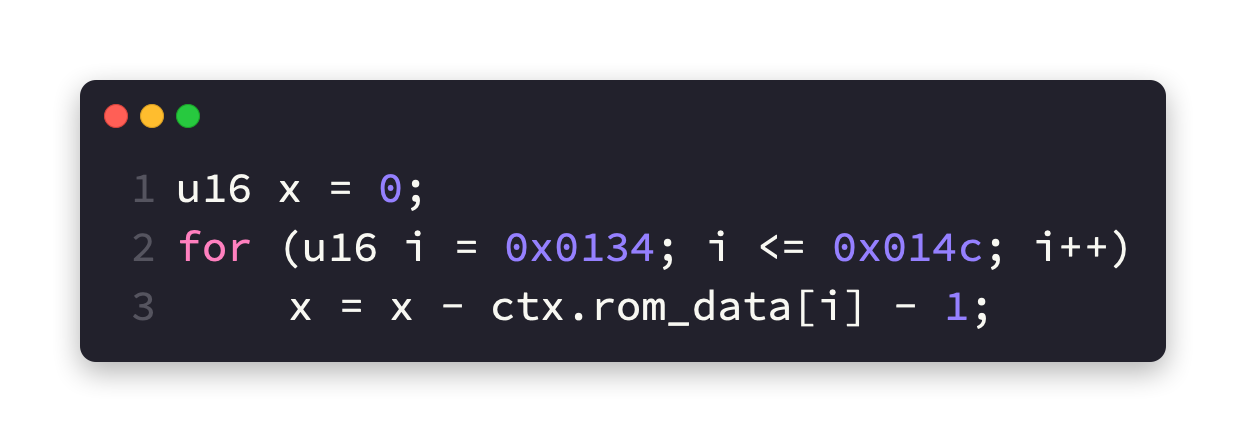
\includegraphics[scale=0.5]{img/checksum.png}
	
	Šajā gadījumā ctx.rom\_data[] ir struktūras masīvs kurā esam ielādējuši ROM faila datus. Pēc cikla izpildes varam salīdzināt mainīgo x ar pašu čeksummu, jeb pašas čeksumas apakšējajaiem 8 bitiem. Ja šajā gadījumā čeksummas nesakrīt tad Kartridžu nevar lādēt.
	
	\pagebreak
	\subsubsection{Kārtridžas ielāde}
	
	Pašus kārtridžas datus ielādējam nodefinētā kontexta struktūrā.
	
	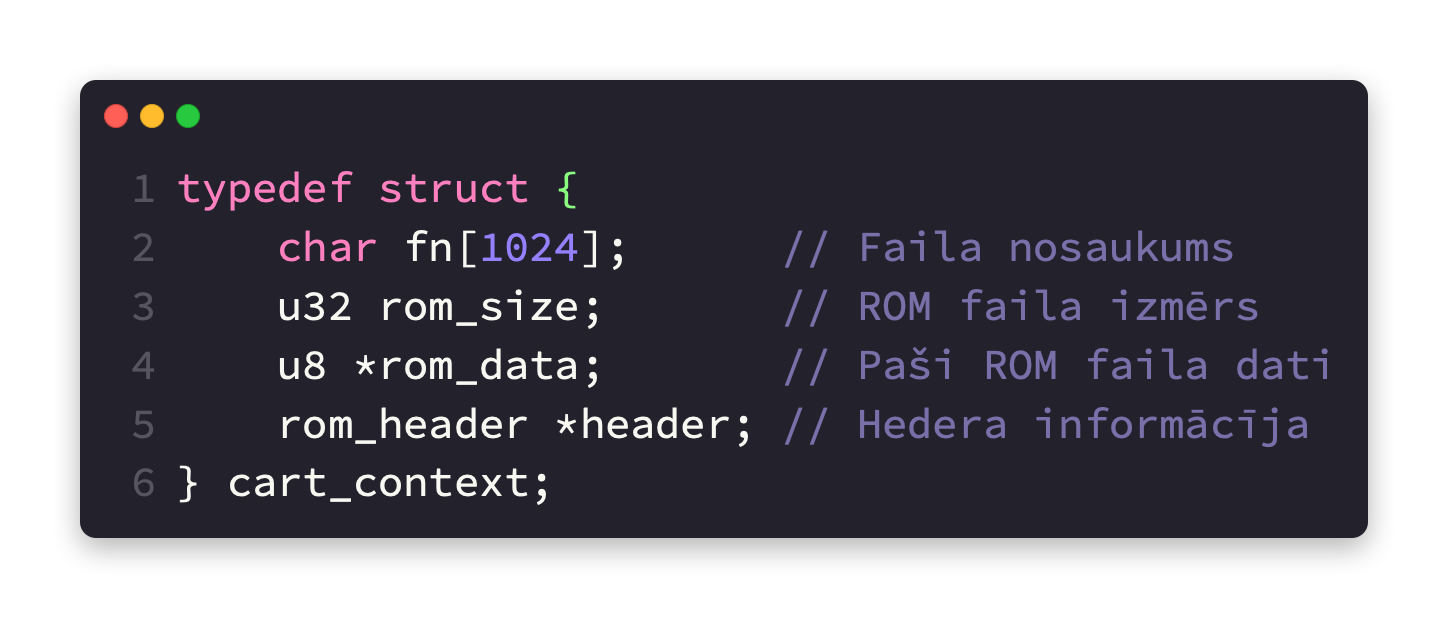
\includegraphics[scale=0.5]{img/structcart.png}
	
	Struktūra sastāv no 4 elementiem, no kuriem viens ir papildus struktūra ar Hedera informācīju.
	
	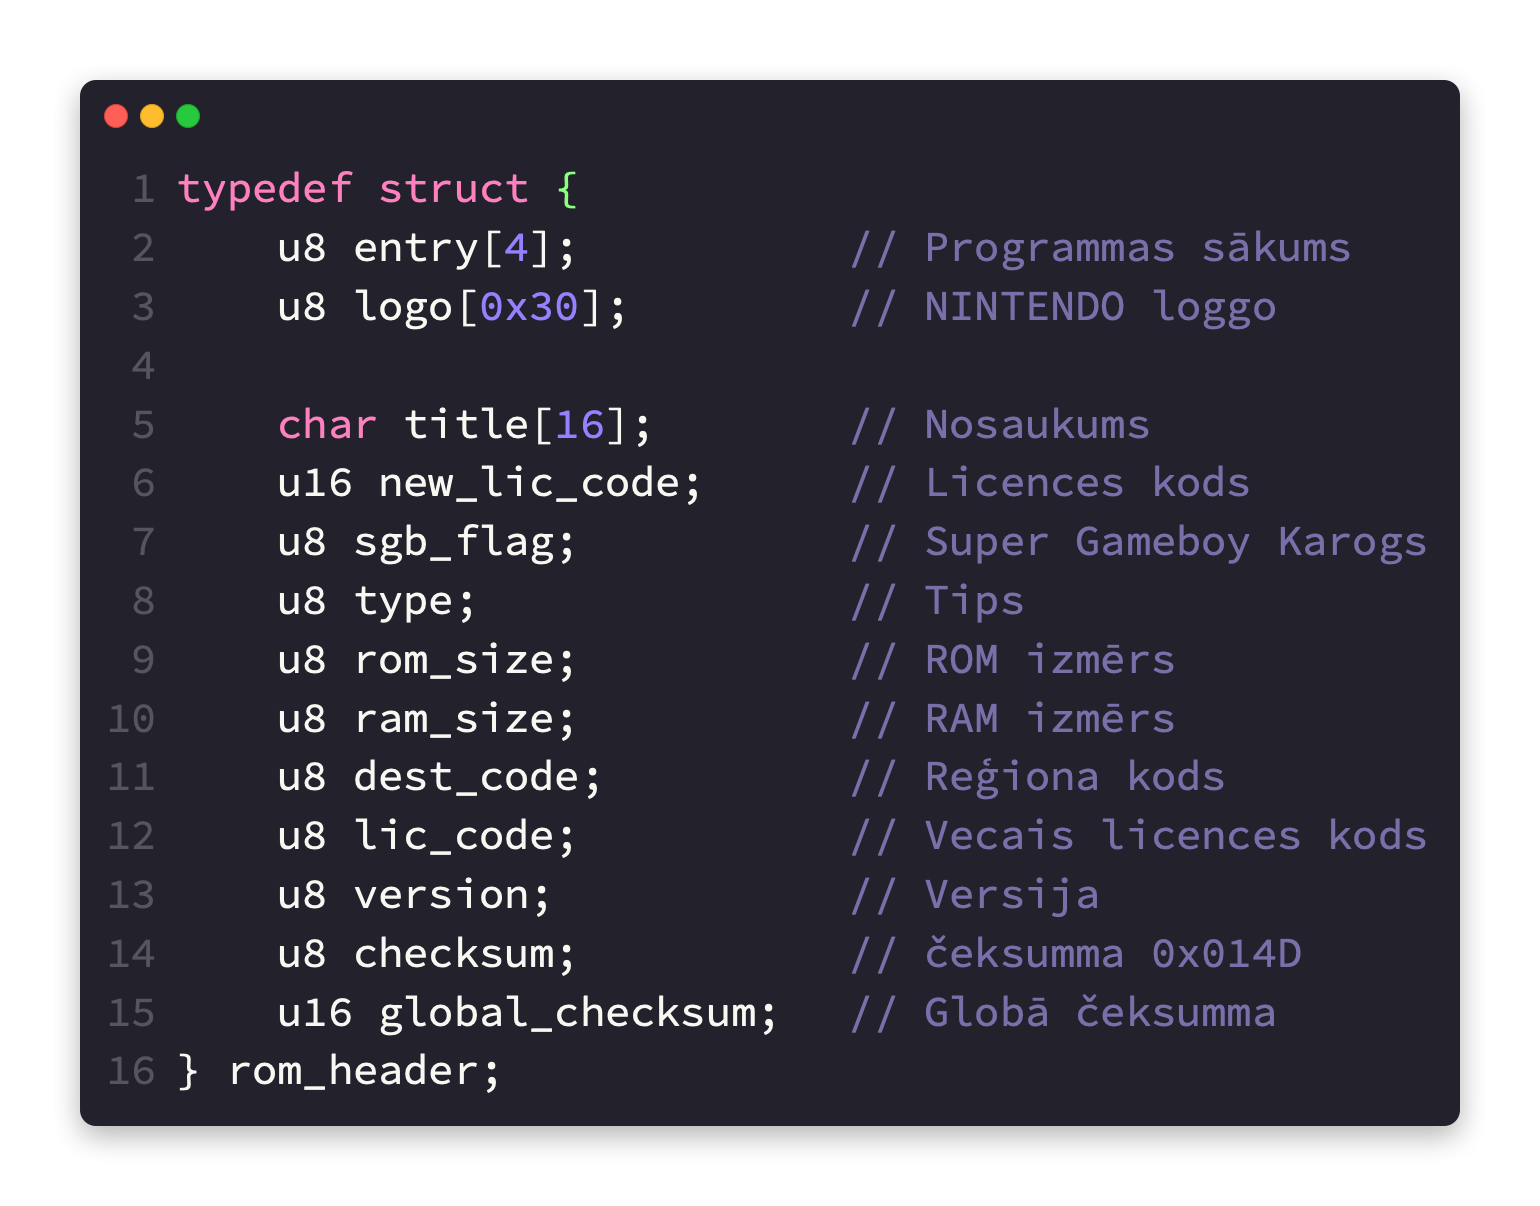
\includegraphics[scale=0.5]{img/rom_header.png}
	
	Kad šīs struktūras tiek aizpildītas ar informācīju varam doties tālāk uz pašu emulācīju un domāt par to kā strādās mūsu emulētais processors.
	\pagebreak
	
	\subsection{Procesora emulācīja}
	Lai effektīvi emulētu procesoru, tas ir principā jaizveido Programmā no jauna. Tas nozīmē ka tam ir jāpilda instrukcījas, jāizmanto reģistri, karogi, addresēšanas veidi u.t.t.
	
	\subsubsection{Procesora struktūras}
	Priekš tā mums ir nepieciešams izveidot datu struktūras kas saturētu Procesora kontekstu dotā mirklī.
	
	Priekš tā mums ir pati galvenā procesora struktūra.
	
	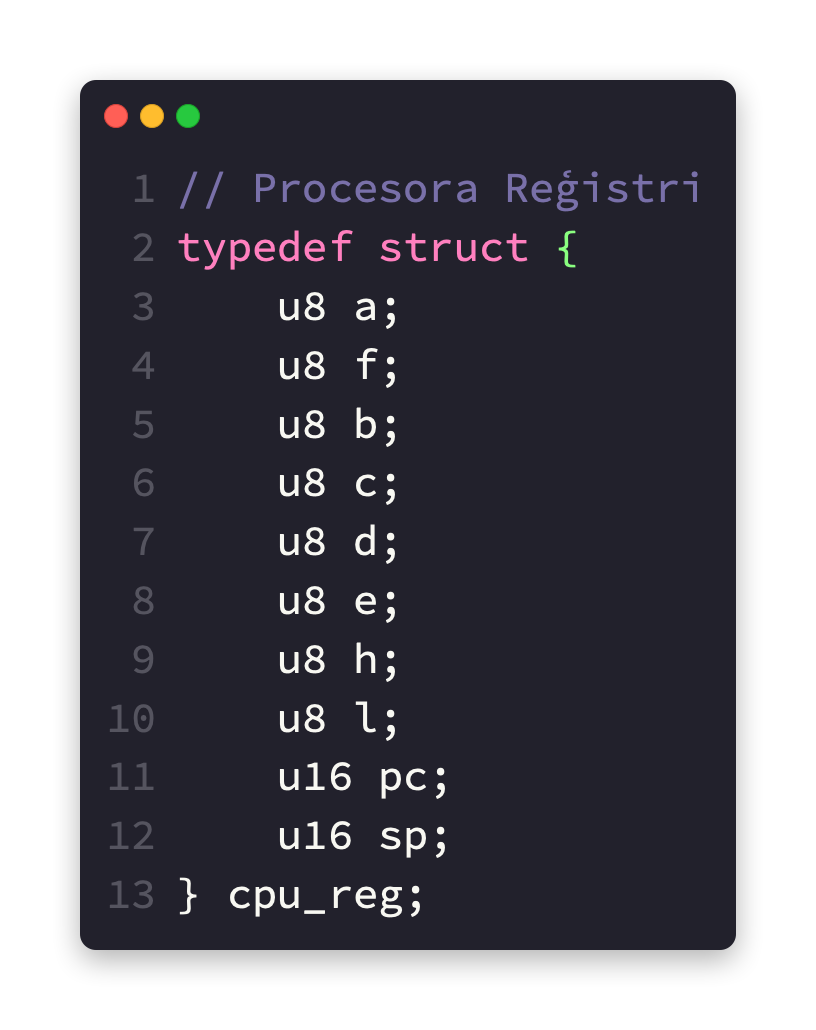
\includegraphics[scale=0.5]{img/reg.png}
	
	Sākam ar procesora reģistriem, realitātē Gameboy procesoram ir 16bitu reģistri, un tie ir tikai 6 (AF, BC, DE,HL, SP, PC) taču par cik pirmie 4 ir dubult reģistri, tad veidojam tos atsevišķi lai atvieglotu savu dzīvi. SP jeb steka rādītājs un PC jeb Programas skaitītājs paliek kā 16bitu skaitļi jo šie divi reģistri tieši ir atbildīgi par procesora adresēšanu. Velviens svarīgs reģistrs ir F, kas ir karogu reģistrs, tas sevī satur 4 karogus, Z, N, H, C. Kur Z ir Nulles karogs, S ir atņemšanas karogs, H ir Pus pārnesuma karogs, un C ir pārnesuma karogs. Tas nozīmē ka mums būs nepieciešams ar Bitu līmeņa operācījām, lai piekļūtu tiem.
	\pagebreak
	
	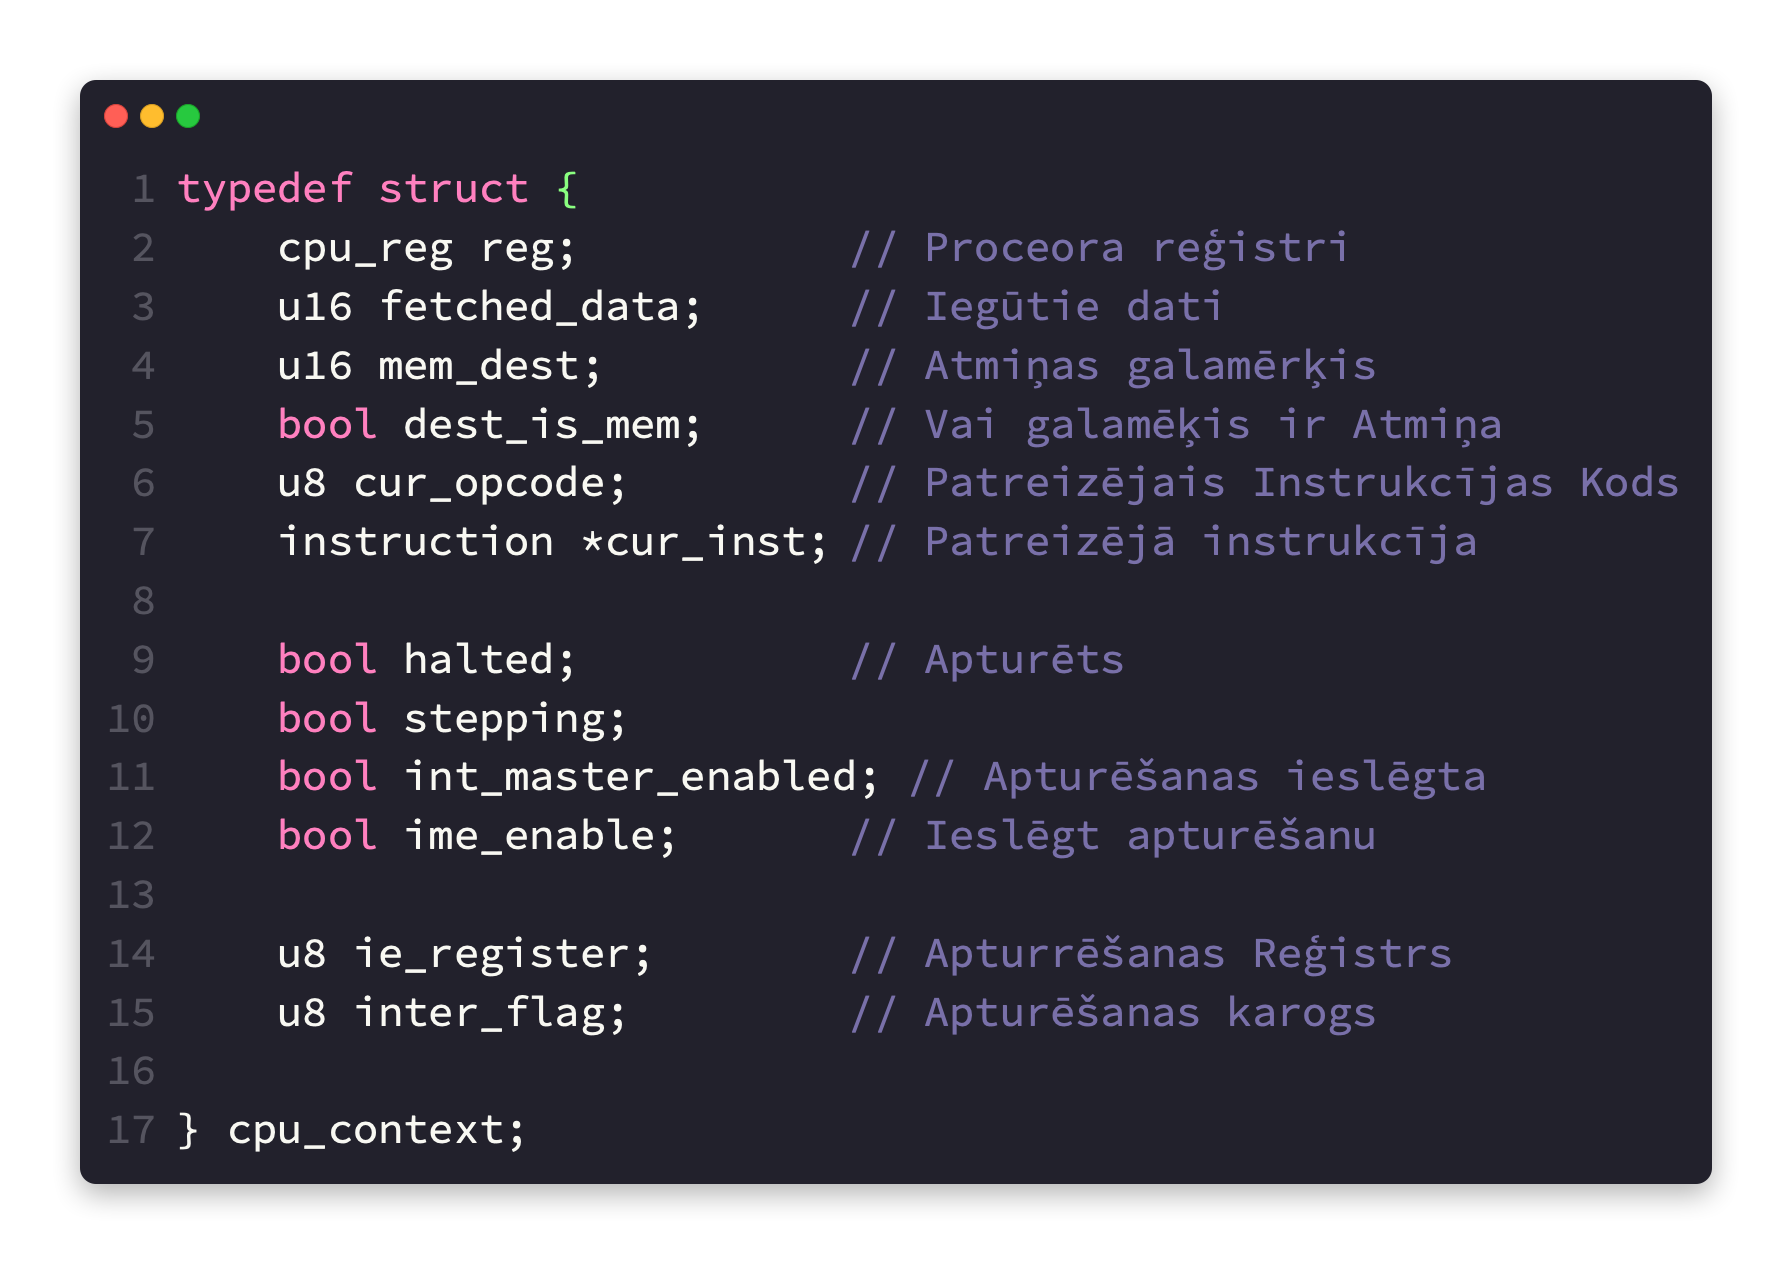
\includegraphics[scale=0.45]{img/cpu_ctx.png}
	
	Šeit ir arī paša procesora konteksta struktūra. Kas satur sevī reģistrus, Apturēšanas funkcionalitātes, instrukcījas u.t.t.
	
	Instrukcīju struktūra sastāv no:
	
	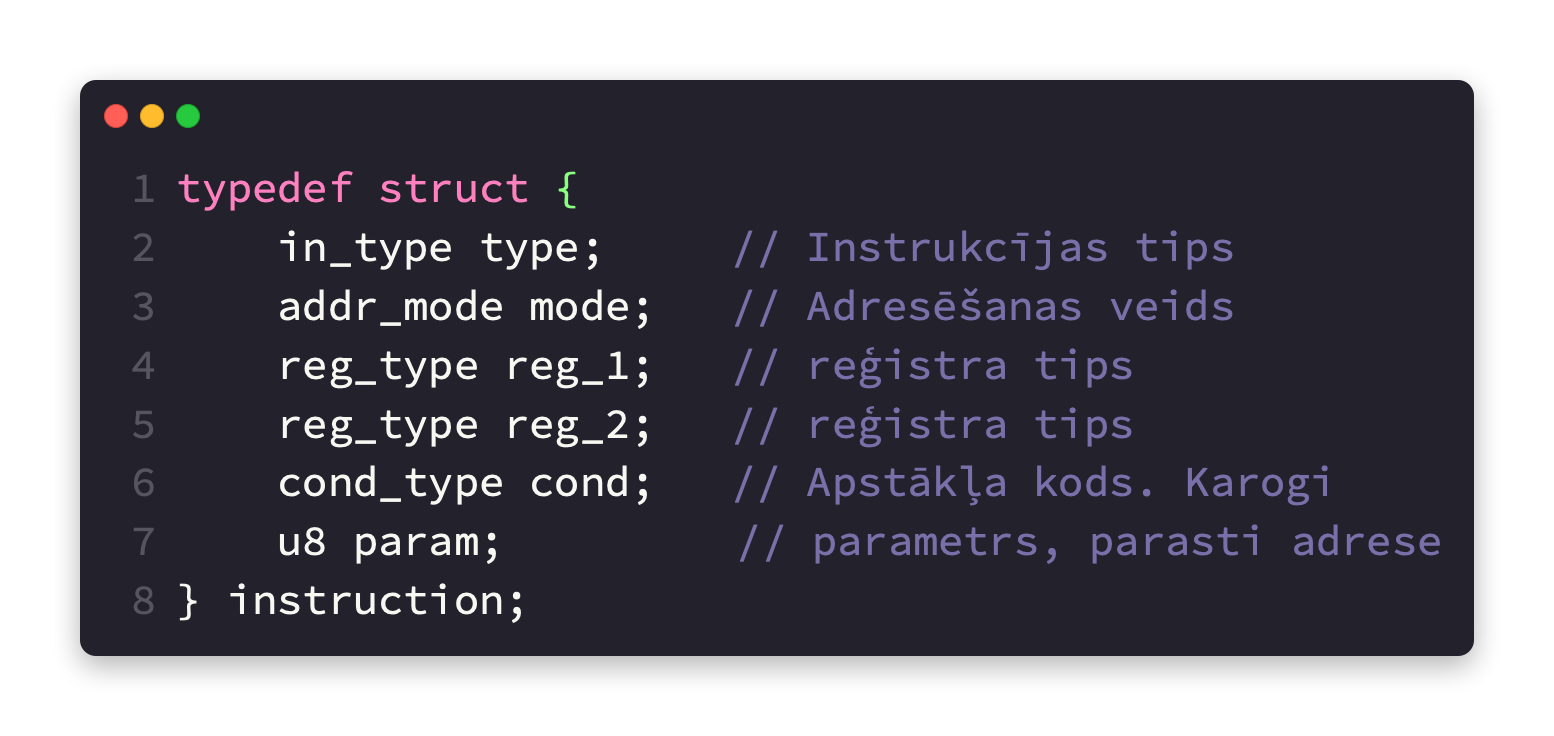
\includegraphics[scale=0.5]{img/instr.png}
	
	Kā redzams, šiš struktūras ir arī lielās problēmu radītājas pie emulācījas, jo struktūras veidojas ļoti sarežģītas un tās kaut, kā vajag arī dabūt līdz funkcījām.
	
	\pagebreak
	
	\subsubsection{Procesora funkcionalitāte}
	
	Emulātors šajā gadījumā iet soli pa solim, pēc Steka Rādītāju un Programas skaitītāju, un tad jau ņem instrukcījas, tās dekodē, atrod pareizo instrukcīju pēc konteksta, un to izpilda.
	
	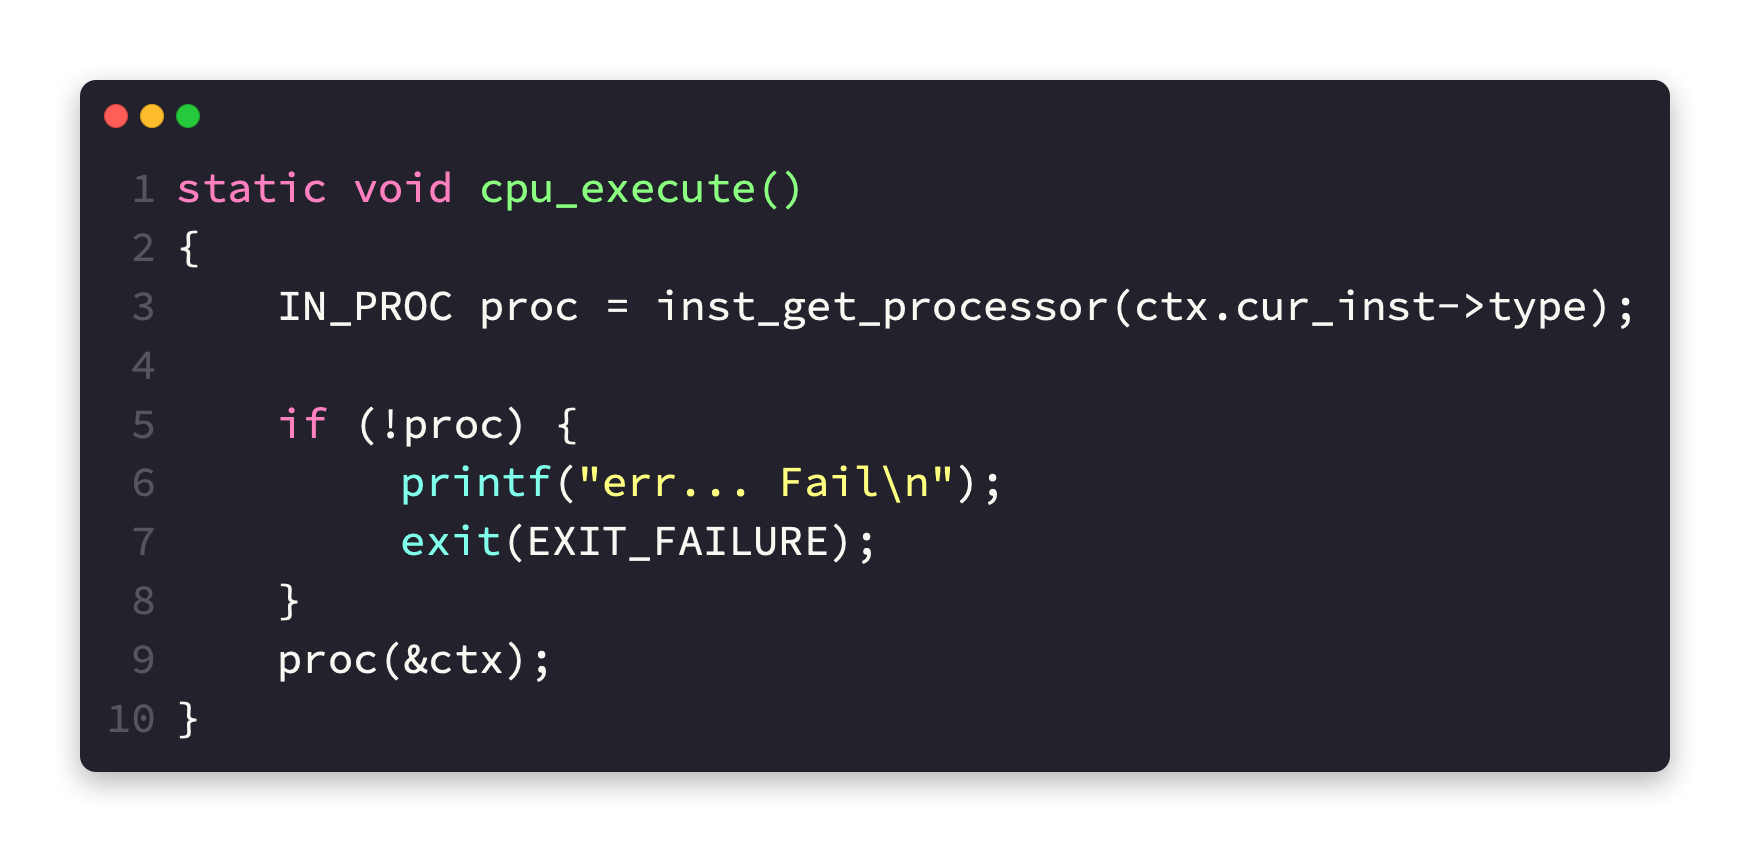
\includegraphics[scale=0.5]{img/cpu_exec.png}
	
	Šeit izveidojam, funkcījas rādītāju, ja neizdodās izveidot rodas programmas kļūda. Tam pēctam padodam kontekstu. 
	
	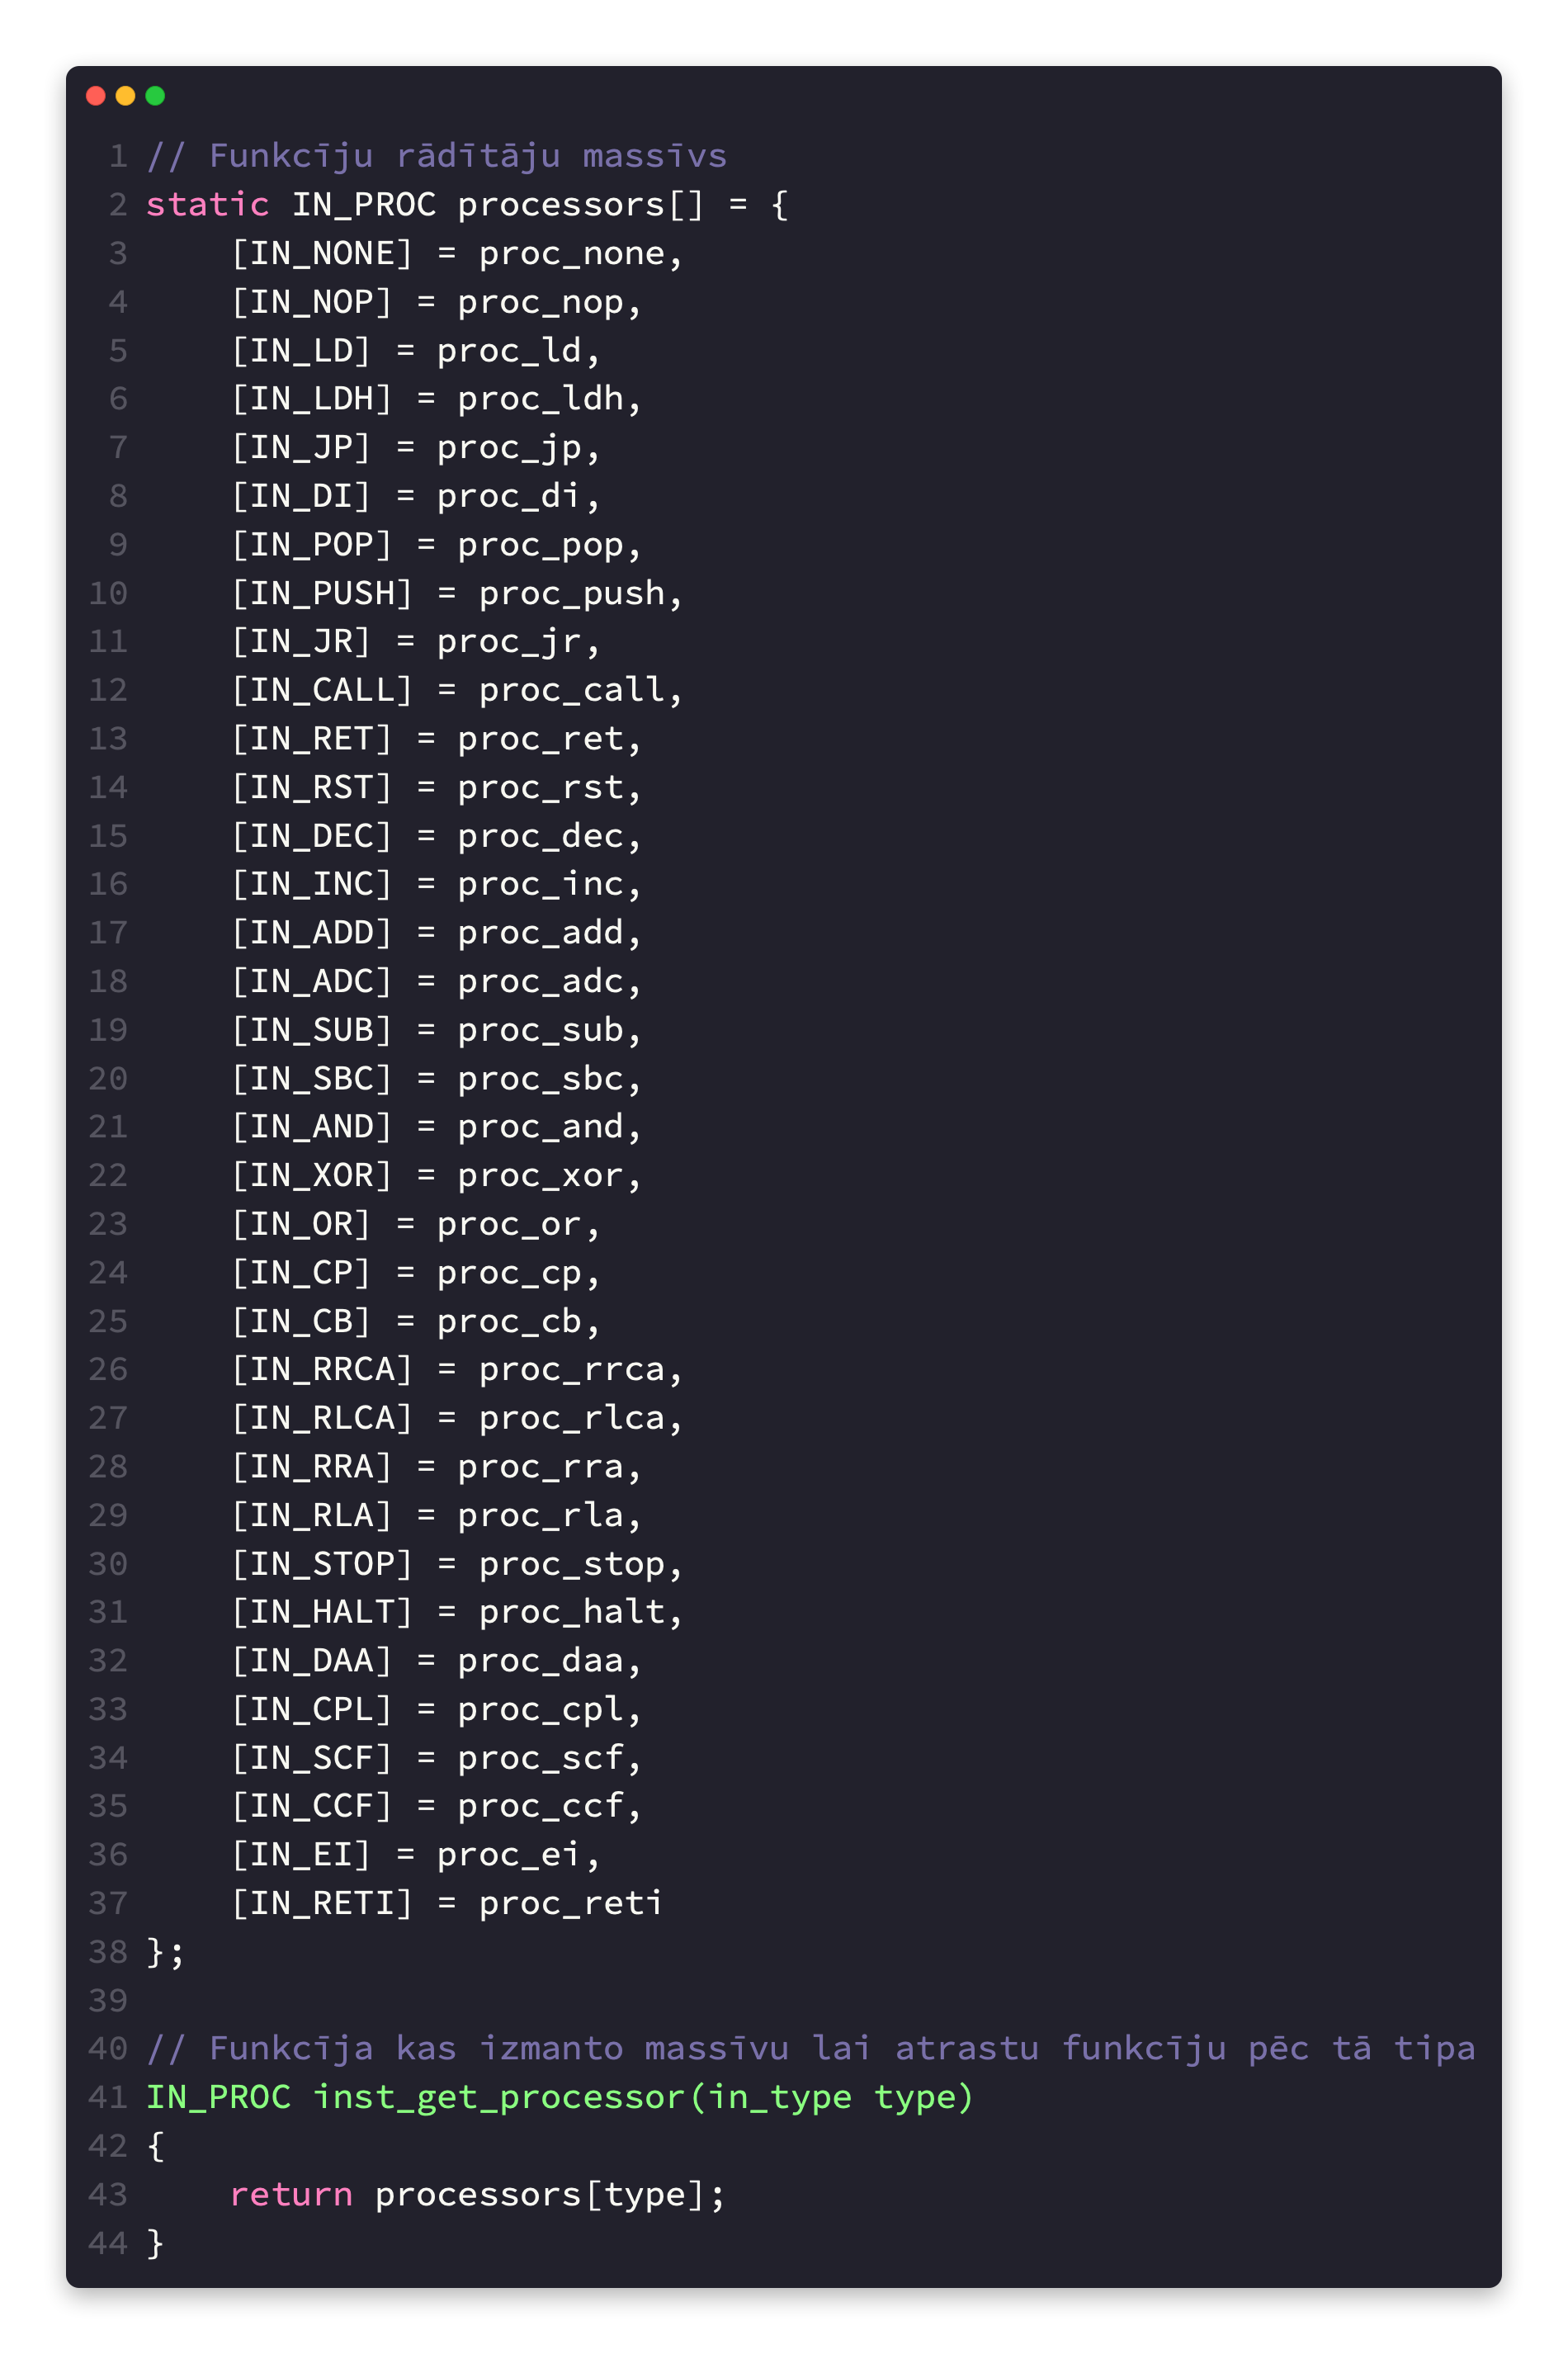
\includegraphics[scale=0.25]{img/instrproc.png}
	
	Šeit var redzēt kā pēc instrukcīju tipa tiek izsaukta pareizā funkcīja. Kas tālāk jau veic darbības pēc paplašināta konteksta un informācījas par instrukciju.
	
	\pagebreak
	
	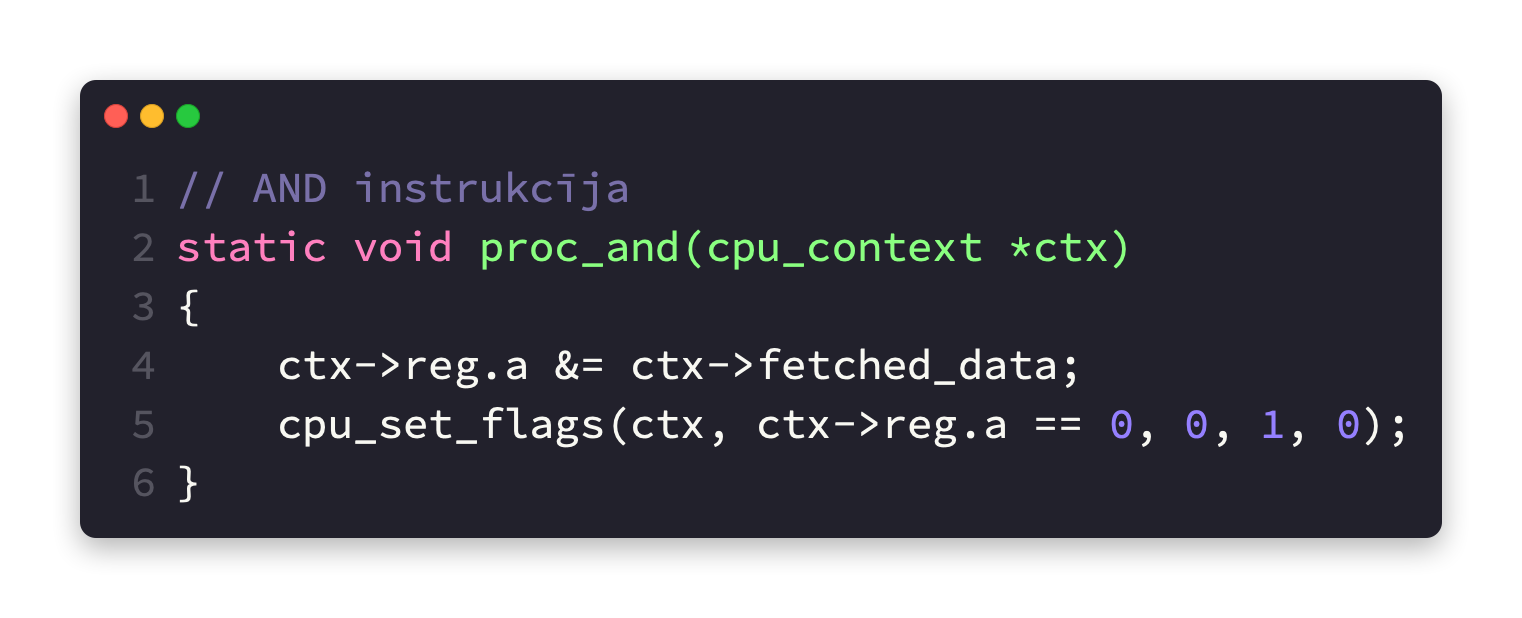
\includegraphics[scale=0.5]{img/instrand.png}
	
	Šeit redzams kā tiek veikta and operācīja Vicam bitu līmeņa AND operācīju ko saglabājam tur pat A reģistrā, ieslēdzam nepieciešamos karogus un ar to and operācīja ir izpildīta.
	
	\subsection{Emulātora status}
	Kopumā emulātora izveide ir sarežģīts uzdevums. Uz doto mirkli Emulātors strādā ar daudz kļūdām un tam nav skaņas. taču tas spēj ielādēt ROM failu, un spēj palaist to. Taču rodās artefakti grafiskajā izdevē un daži ROM faili, aptur Emulātora darbību.
	
	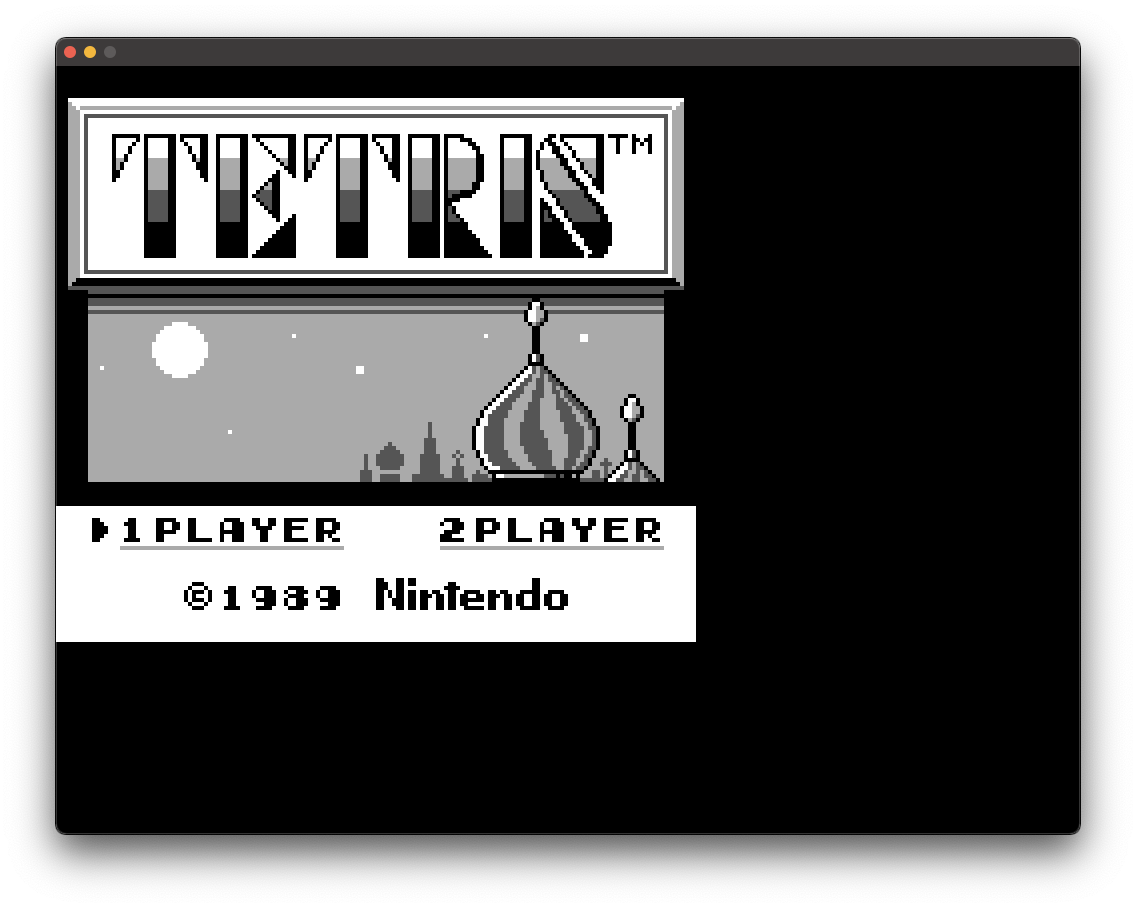
\includegraphics[scale=0.35]{img/gbemutetris.png}
	
	Šeit redzama spēle TETRIS ko izmantoju emulātora testēšanai. Titula ekrāns strādā un izvada ekrānā attēlu bez redzamiem artefaktiem. Taču kad mēģina spēlēt spēli veidojas artevakti, līdz ar to redzams ka emulātors nav līdz galam pabeigts un ir kļūdains.
	
	\pagebreak
	
	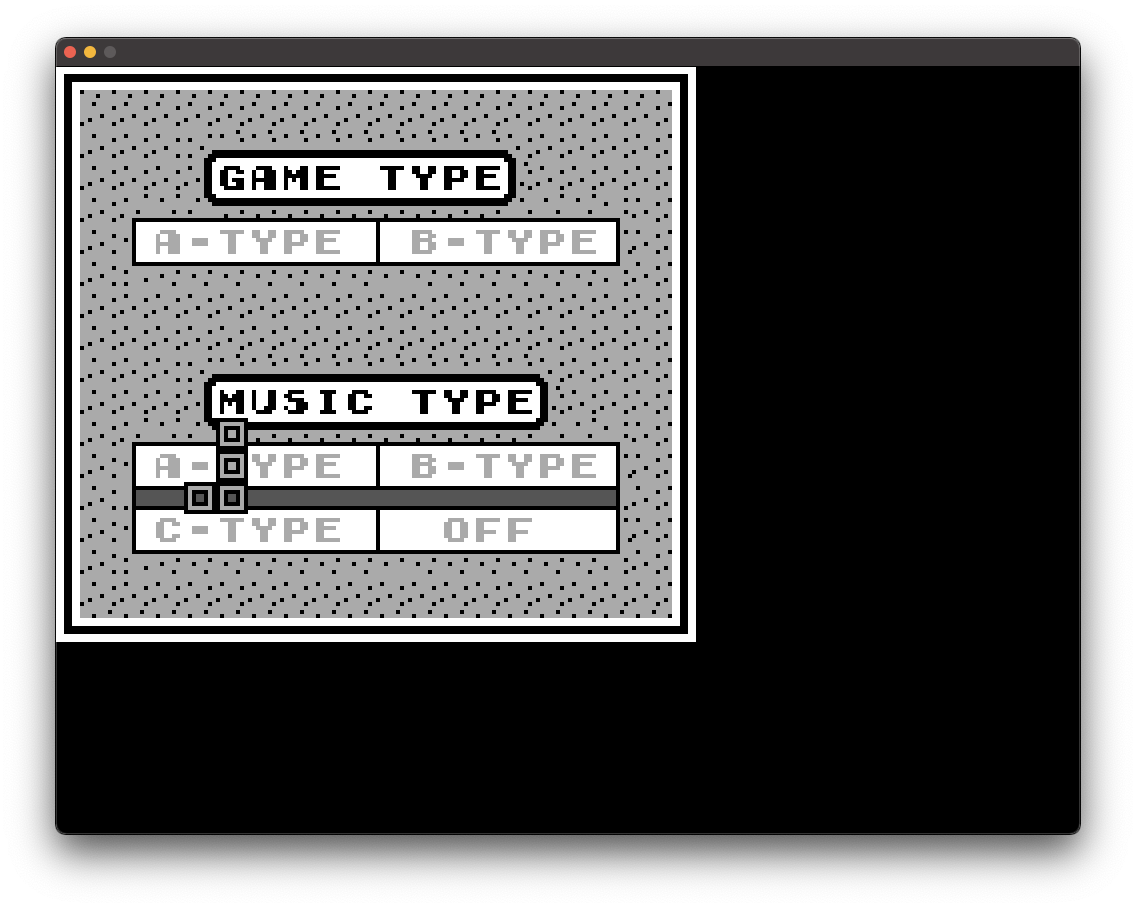
\includegraphics[scale=0.35]{img/gbemutetris2.png}
	
	\section{Secinājumi un ierosinājumi}
	Secinājumi pēc prakses ir vienkārši. Izvēlētais prakses uzdevums iespējams ir par sarežģītu, taču rezultātā esmu uzzinājis arī daudz ko jauni. Uzskatu ka prakse ir aizvadīta veiksmīgi, lai gan tā ir bijusi grūta taču nevarētu teikt, ka tā nav izveusies.
	
	Prakses laikā izdevās izveidot pamata emulācījas programmu priekš Gameboy sistēmas, tā spēj ielādēt ROM failus un spēj veikt pamata Gameboy funkcijas, taču tā nav līdz galam pabeigta, un mēģinot spēlēt, spēles caur emulātoru veidojās dažādi vizuālie artifakti, vai emulātora programa, vienkārši apstāj savu darbību.
	
	Ieteikumi, būtu veidot garāku prakses laiku, it īpaši strādājošajiem studentiem, kam prakses apvienošana ar darbu sagādā sarežģītības.
	
	\pagebreak
	\section{Informācījas avoti}
	
	\href{https://gbdev.io/pandocs/About.html}{Gameboy Izstrādes dokuments.}
	
	\href{https://www.copetti.org/writings/consoles/game-boy/}{Informācīja par Gameboy}
	
	\href{https://www.pastraiser.com/cpu/gameboy/gameboy_opcodes.html}{Infromācīja par Gameboy instrukcījām}
	
	\href{https://emulation.gametechwiki.com/index.php/Game_Boy/Game_Boy_Color_emulators}{Informācīja par GameBoy Emulācīju}
	
	\href{https://en.wikipedia.org/wiki/Emulator}{Informācīja par Emulātoriem}
	
	\href{https://en.wikipedia.org/wiki/Game_Boy}{Informācīja par Gameboy Wikipedia}
	
	\href{https://en.wikipedia.org/wiki/Unix}{Informācīja par UNIX}
	
	\href{https://en.wikipedia.org/wiki/Linux}{Informācīja par Linux}
	
	\href{https://en.wikipedia.org/wiki/Emacs}{Informācīja par Emacs}
	
	\href{https://www.vdi.gov.lv/sites/vdi/files/media_file/2_2_12_ergonomika_un_ergonomiskie_darba_vides_riska_faktori.pdf}{informācīja par Ergonomiku}
	
\end{document}
